% Options for packages loaded elsewhere
\PassOptionsToPackage{unicode}{hyperref}
\PassOptionsToPackage{hyphens}{url}
%
\documentclass[
  man]{apa6}
\usepackage{amsmath,amssymb}
\usepackage{lmodern}
\usepackage{iftex}
\ifPDFTeX
  \usepackage[T1]{fontenc}
  \usepackage[utf8]{inputenc}
  \usepackage{textcomp} % provide euro and other symbols
\else % if luatex or xetex
  \usepackage{unicode-math}
  \defaultfontfeatures{Scale=MatchLowercase}
  \defaultfontfeatures[\rmfamily]{Ligatures=TeX,Scale=1}
\fi
% Use upquote if available, for straight quotes in verbatim environments
\IfFileExists{upquote.sty}{\usepackage{upquote}}{}
\IfFileExists{microtype.sty}{% use microtype if available
  \usepackage[]{microtype}
  \UseMicrotypeSet[protrusion]{basicmath} % disable protrusion for tt fonts
}{}
\makeatletter
\@ifundefined{KOMAClassName}{% if non-KOMA class
  \IfFileExists{parskip.sty}{%
    \usepackage{parskip}
  }{% else
    \setlength{\parindent}{0pt}
    \setlength{\parskip}{6pt plus 2pt minus 1pt}}
}{% if KOMA class
  \KOMAoptions{parskip=half}}
\makeatother
\usepackage{xcolor}
\usepackage{graphicx}
\makeatletter
\def\maxwidth{\ifdim\Gin@nat@width>\linewidth\linewidth\else\Gin@nat@width\fi}
\def\maxheight{\ifdim\Gin@nat@height>\textheight\textheight\else\Gin@nat@height\fi}
\makeatother
% Scale images if necessary, so that they will not overflow the page
% margins by default, and it is still possible to overwrite the defaults
% using explicit options in \includegraphics[width, height, ...]{}
\setkeys{Gin}{width=\maxwidth,height=\maxheight,keepaspectratio}
% Set default figure placement to htbp
\makeatletter
\def\fps@figure{htbp}
\makeatother
\setlength{\emergencystretch}{3em} % prevent overfull lines
\providecommand{\tightlist}{%
  \setlength{\itemsep}{0pt}\setlength{\parskip}{0pt}}
\setcounter{secnumdepth}{-\maxdimen} % remove section numbering
% Make \paragraph and \subparagraph free-standing
\ifx\paragraph\undefined\else
  \let\oldparagraph\paragraph
  \renewcommand{\paragraph}[1]{\oldparagraph{#1}\mbox{}}
\fi
\ifx\subparagraph\undefined\else
  \let\oldsubparagraph\subparagraph
  \renewcommand{\subparagraph}[1]{\oldsubparagraph{#1}\mbox{}}
\fi
\newlength{\cslhangindent}
\setlength{\cslhangindent}{1.5em}
\newlength{\csllabelwidth}
\setlength{\csllabelwidth}{3em}
\newlength{\cslentryspacingunit} % times entry-spacing
\setlength{\cslentryspacingunit}{\parskip}
\newenvironment{CSLReferences}[2] % #1 hanging-ident, #2 entry spacing
 {% don't indent paragraphs
  \setlength{\parindent}{0pt}
  % turn on hanging indent if param 1 is 1
  \ifodd #1
  \let\oldpar\par
  \def\par{\hangindent=\cslhangindent\oldpar}
  \fi
  % set entry spacing
  \setlength{\parskip}{#2\cslentryspacingunit}
 }%
 {}
\usepackage{calc}
\newcommand{\CSLBlock}[1]{#1\hfill\break}
\newcommand{\CSLLeftMargin}[1]{\parbox[t]{\csllabelwidth}{#1}}
\newcommand{\CSLRightInline}[1]{\parbox[t]{\linewidth - \csllabelwidth}{#1}\break}
\newcommand{\CSLIndent}[1]{\hspace{\cslhangindent}#1}
\ifLuaTeX
\usepackage[bidi=basic]{babel}
\else
\usepackage[bidi=default]{babel}
\fi
\babelprovide[main,import]{english}
% get rid of language-specific shorthands (see #6817):
\let\LanguageShortHands\languageshorthands
\def\languageshorthands#1{}
% Manuscript styling
\usepackage{upgreek}
\captionsetup{font=singlespacing,justification=justified}

% Table formatting
\usepackage{longtable}
\usepackage{lscape}
% \usepackage[counterclockwise]{rotating}   % Landscape page setup for large tables
\usepackage{multirow}		% Table styling
\usepackage{tabularx}		% Control Column width
\usepackage[flushleft]{threeparttable}	% Allows for three part tables with a specified notes section
\usepackage{threeparttablex}            % Lets threeparttable work with longtable

% Create new environments so endfloat can handle them
% \newenvironment{ltable}
%   {\begin{landscape}\centering\begin{threeparttable}}
%   {\end{threeparttable}\end{landscape}}
\newenvironment{lltable}{\begin{landscape}\centering\begin{ThreePartTable}}{\end{ThreePartTable}\end{landscape}}

% Enables adjusting longtable caption width to table width
% Solution found at http://golatex.de/longtable-mit-caption-so-breit-wie-die-tabelle-t15767.html
\makeatletter
\newcommand\LastLTentrywidth{1em}
\newlength\longtablewidth
\setlength{\longtablewidth}{1in}
\newcommand{\getlongtablewidth}{\begingroup \ifcsname LT@\roman{LT@tables}\endcsname \global\longtablewidth=0pt \renewcommand{\LT@entry}[2]{\global\advance\longtablewidth by ##2\relax\gdef\LastLTentrywidth{##2}}\@nameuse{LT@\roman{LT@tables}} \fi \endgroup}

% \setlength{\parindent}{0.5in}
% \setlength{\parskip}{0pt plus 0pt minus 0pt}

% Overwrite redefinition of paragraph and subparagraph by the default LaTeX template
% See https://github.com/crsh/papaja/issues/292
\makeatletter
\renewcommand{\paragraph}{\@startsection{paragraph}{4}{\parindent}%
  {0\baselineskip \@plus 0.2ex \@minus 0.2ex}%
  {-1em}%
  {\normalfont\normalsize\bfseries\itshape\typesectitle}}

\renewcommand{\subparagraph}[1]{\@startsection{subparagraph}{5}{1em}%
  {0\baselineskip \@plus 0.2ex \@minus 0.2ex}%
  {-\z@\relax}%
  {\normalfont\normalsize\itshape\hspace{\parindent}{#1}\textit{\addperi}}{\relax}}
\makeatother

% \usepackage{etoolbox}
\makeatletter
\patchcmd{\HyOrg@maketitle}
  {\section{\normalfont\normalsize\abstractname}}
  {\section*{\normalfont\normalsize\abstractname}}
  {}{\typeout{Failed to patch abstract.}}
\patchcmd{\HyOrg@maketitle}
  {\section{\protect\normalfont{\@title}}}
  {\section*{\protect\normalfont{\@title}}}
  {}{\typeout{Failed to patch title.}}
\makeatother

\usepackage{xpatch}
\makeatletter
\xapptocmd\appendix
  {\xapptocmd\section
    {\addcontentsline{toc}{section}{\appendixname\ifoneappendix\else~\theappendix\fi\\: #1}}
    {}{\InnerPatchFailed}%
  }
{}{\PatchFailed}
\keywords{FIXME\newline\indent Word count: FIXME}
\DeclareDelayedFloatFlavor{ThreePartTable}{table}
\DeclareDelayedFloatFlavor{lltable}{table}
\DeclareDelayedFloatFlavor*{longtable}{table}
\makeatletter
\renewcommand{\efloat@iwrite}[1]{\immediate\expandafter\protected@write\csname efloat@post#1\endcsname{}}
\makeatother
\usepackage{lineno}

\linenumbers
\usepackage{csquotes}
\ifLuaTeX
  \usepackage{selnolig}  % disable illegal ligatures
\fi
\IfFileExists{bookmark.sty}{\usepackage{bookmark}}{\usepackage{hyperref}}
\IfFileExists{xurl.sty}{\usepackage{xurl}}{} % add URL line breaks if available
\urlstyle{same} % disable monospaced font for URLs
\hypersetup{
  pdftitle={Replicability of US-China differences in cognition and perception across 12 tasks},
  pdfauthor={Anjie Cao*1, Alexandra Carstensen*2, Shan Gao3, \& Michael C. Frank1},
  pdflang={en-EN},
  pdfkeywords={FIXME},
  hidelinks,
  pdfcreator={LaTeX via pandoc}}

\title{Replicability of US-China differences in cognition and perception across 12 tasks}
\author{Anjie Cao*\textsuperscript{1}, Alexandra Carstensen*\textsuperscript{2}, Shan Gao\textsuperscript{3}, \& Michael C. Frank\textsuperscript{1}}
\date{}


\shorttitle{Replicate US-China differences}

\authornote{

We gratefully acknowledge Alvin Tan, Joseph Outa, and the members of the Language and Cognition Lab at Stanford for comments and assistance. Experiment 1 was previously reported in abbreviated form in the Proceedings of the Cognitive Science Society as Carstensen et al.~(2020).

Correspondence concerning this article should be addressed to Anjie Cao*, 450 Jane Stanford Way, Stanford, 94305. E-mail: \href{mailto:anjiecao@stanford.edu}{\nolinkurl{anjiecao@stanford.edu}}

}

\affiliation{\vspace{0.5cm}\textsuperscript{1} Department of Psychology, Stanford University\\\textsuperscript{2} Department of Psychology, University of California, San Diego\\\textsuperscript{3} FIXME}

\abstract{%
Cultural differences between the US and China have been investigated using a broad array of psychological tasks measuring differences between cognition, language, perception, and reasoning. We conducted two large-scale replications of a selection of 12 tasks previously reported to show cross-cultural differences, using online convenience samples of adults. Five of these tasks showed robust cross-cultural differences, while six showed no difference and one showed a small difference in the opposite direction. Tasks showing cross-cultural differences tended to have multiple trials measuring high-level reasoning and language; those that did not show cross-cultural difference included measures of attention/perception, implicit social processes, or were initially designed to show differences in children. As in prior work, cross-cultural differences in cognition (in those tasks showing differences) were not strongly related to explicit measures of cultural identity and behavior.
}



\begin{document}
\maketitle

\hypertarget{introduction}{%
\section{Introduction}\label{introduction}}

Cross-cultural differences are a striking part of the broader landscape of human variation. Differences in values and behavior across cultures are obvious to even a casual observer, and researchers have attempted to quantify these differences via a wide range of measures. Comparisons between the United States and China -- often as exemplars of Western and East Asian cultures -- have been especially well-researched, with differences attested in a wide range of cognitive domains, including visual attention (Chua, Boland, \& Nisbett, 2005; Ji, Peng, \& Nisbett, 2000; Waxman et al., 2016), executive function (Sabbagh, Xu, Carlson, Moses, \& Lee, 2006; Tan, 2020), language learning (Chan et al., 2011, 2011; Tardif, 1996; Waxman et al., 2016), relational reasoning (Carstensen et al., 2019; Cheng, 2020; Richland, Chan, Morrison, \& Au, 2010; Su, 2020), similarity judgments (Ji, Zhang, \& Nisbett, 2004), values (Ji, Nisbett, \& Su, 2001; Kwan, Bond, \& Singelis, 1997; Spencer-Rodgers, Williams, Hamilton, Peng, \& Wang, 2007), preferences (Corriveau et al., 2017; DiYanni, Corriveau, Kurkul, Nasrini, \& Nini, 2015; Liang \& He, 2012) and self-concepts (Spencer-Rodgers, Boucher, Mori, Wang, \& Peng, 2009; Spencer-Rodgers, Boucher, Peng, \& Wang, 2009). As a result, the US and China are increasingly becoming major cultural poles in efforts to assess and measure cultural differences (Muthukrishna et al., 2020) and correct for the pervasive bias in psychology research toward US and European samples (Arnett, 2016; Henrich, Heine, \& Norenzayan, 2010; Nielsen, Haun, Kärtner, \& Legare, 2017).

Despite a long empirical tradition of comparisons between these two cultures and an abundance of psychological accounts for observed differences, there is little consensus on how measurements relate to each other. Reports of cultural differences are often difficult to compare quantitatively because of the varying samples, measures, and methods used in different reports. Further, many of the most prominent reports of cross-cultural differences predate the field-wide discussion of methodological issues in psychology research during the past 10 years (Open Science Collaboration, 2015). For example, much research in this tradition has been exploratory and hence has not followed current guidance regarding limiting analytic flexibility in order to decrease false positives (Simmons, Nelson, \& Simonsohn, 2011). Given the importance of claims about specific cross-cultural differences for constructing theories of culture more broadly (e.g., Markus \& Kitayama, 1992, 2010), replication of many empirical findings is likely warranted.

There is already some empirical evidence suggesting issues in the robustness of cross-cultural measurements. measures used in this literature are not standardized and do not have published evidence about reliability and validity (Flake \& Fried, 2020). The few extant direct comparisons between measures of cultural difference suggest that theoretically related tasks, such as implicit and explicit measures of the same construct, often do not cohere (e.g., Kitayama, Park, Sevincer, Karasawa, \& Uskul, 2009). Further, in a study with twenty cross-cultural measures used within a single US sample, Na et al. (2010) found a lack of coherence between tasks measuring social orientation and cognitive style, observing only 8 significant correlations between tasks across 90 statistical tests \footnote{ The authors interpret their findings as imply the measures are orthogonal -- indexing different constructs -- and conclude that group-level differences between cultures are unlikely to relate to within-group individual differences. However an alternative possibility is that the reliabilities of many individual tasks are low, a feature which would ensure low correlations between them.
  .}. Further, more recent work has raised concerns about low external validity of some cross-cultural measures and failed to replicate cultural differences on several related measures (Mercier, Yama, Kawasaki, Adachi, \& Van der Henst, 2012; Mercier, Zhang, Qu, Lu, \& Van der Henst, 2015; Zhou, Gotch, Zhou, \& Liu, 2008). Thus, there is a need for exploration of the reliability of individual tasks as well as the intercorrelations between them.

Our goal in the current study was to replicate a set of cross-cultural measures that had previously been used in comparisons of East Asian and Western cultures (most often comparisons between US and either Chinese or Japanese participants). We made the decision to pursue the strategy of gathering relatively large and heterogeneous convenience samples using online recruitment, rather than recruiting smaller, more matched samples using in-lab recruitment. Our reasoning was that the larger samples that we could access using online recruitment would allow us to conduct highly-powered statistical tests, allowing us to either reject or accept the null hypothesis of no cultural difference between measures. Further, larger samples would afford the analysis of individual and demographic differences within culture, a topic of considerable interest in this literature (e.g., Na et al., 2010). Finally, the development of browser-based online versions of prominent cross-cultural tasks would allow their inspection and reuse by other researchers, thus promoting a more cumulative approach to the measurement of cultural differences.

The interpretation of any replication result is complex, given that disparate outcomes between an initial study and a replication can occur for many reasons -- including but not limited to differences in experimental methods, sample or population differences, and simple sampling variation in the outcomes Machery (2020). Our strategy of pursuing online convenience samples limits the interpretation of our replication results: nearly all of the tasks we selected had previously been administered in person, and the populations sampled in previous reports varied but were largely convenience samples of either college students or community members. More generally, our strategy of constructing a battery of replication studies and administering them uniformly means that specific decisions about sampling and administration will not be matched with the original studies (which were likely heterogeneous in their samples and administration). Thus, our replication studies should be taken as an assessment of whether a set of previously-reported cross-cultural differences can be recovered in convenience populations recruited online, rather than as assessments of the veracity of the original findings. Nevertheless, we believe that the field of cross-cultural psychology can be advanced via the identification of tasks that yield cross-cultural differences robustly across a variety of samples and administration formats and we hope our work contributes to this aim. We return to this interpretive issue in the General Discussion.

Our task selection process was initially shaped by an interest in relational reasoning and accounts explaining it with reference to cross-cultural differences in visual attention and social cognition (Duffy, Toriyama, Itakura, \& Kitayama, 2009; e.g., Kuwabara \& Smith, 2012; Moriguchi, Evans, Hiraki, Itakura, \& Lee, 2012). Additionally, in Experiment 1, we selected tasks that could potentially be administered to young children as well as adults, for use in future work addressing developmental questions about the relative time course of cross-cultural differences across the visual, social, and cognitive domains. We balanced four desiderata in our task selection, preferentially choosing tasks that (1) had been theoretically or empirically implicated in relational reasoning, (2) were associated with differential performance in US-China comparisons or related cultural contrasts (e.g., East Asian vs.~Western cultures), (3) were relatively short, accessible tasks appropriate for web administration, and (4) were vision or social cognition accounts for relational reasoning. We further conducted a fairly extensive set of pilots to ensure that participants understood instructions and that the tasks yielded interpretable data.

In Experiment 2, we selected a second set of tasks to investigate based in part on the results of Experiment 1. In particular, we repeated a handful of tasks from Experiment 1 to collect further evidence (in some cases, varying task parameters). We then selected a further set of tasks that probed both cross-cultural differences in higher-level cognition (e.g., language and reasoning) and perception, again respecting the desideratum that the tasks should be relatively short and amenable to administration in a web browser. The final set of tasks included in each Experiment is listed in Table 1.

In addition to the goal of replicating individual tasks in which cross-cultural differences in cognition and perception had been previously reported, our hope was that the relatively large dataset that we collected could be used to explore the structure of within- and across-cultural variation in cognition and perception more broadly. Towards this goal, we included a relatively extensive demographic questionnaire in both of our Experiments, with the aim of using these measures to explore variation within our samples. In the final section of the paper, we report a series of exploratory analyses. The first of these assess the reliability of individual tasks, aiming to gauge whether individual tasks are reliable enough from a psychometric point of view to support further individual differences analyses. We then report across-task correlations, aiming to discover covariation between tasks that might indicate that they load on the same construct. Finally, we turn to analyses of whether within-culture demographic variables predict variation in task performance. Overall, a number of tasks revealed acceptable levels of reliability, and tasks clustered together FIXMEXYZ FIXME. We found relatively limited evidence for demographic predictors of within-culture variation, however.

We make all code and data from our experiments available for further data collection and analysis in hopes of promoting further cumulative work on measures and theories of cross-cultural variation.

\hypertarget{experiment-1}{%
\section{Experiment 1}\label{experiment-1}}

In Experiment 1, our goal was to evaluate cross-cultural differences in a variety of constructs. We assembled a web-based battery of tasks and tested these on a snowball sample of US and Chinese participants.

\hypertarget{methods}{%
\subsection{Methods}\label{methods}}

\hypertarget{participants}{%
\subsubsection{Participants}\label{participants}}

We recruited participants through snowball sampling seeded at large universities in the US and China, in which participants directly recruited by the researchers were encouraged to recruit their friends and family members through email forwarding and social media sharing. Participants in the US were compensated with \$5 gift certificates (USD) and participants in China received ¥35 (CNY).

We recruited 203 and 201 participants each from the US and China, respectively. Since we did not have strong a priori expectations about specific effect sizes, our overall preregistered sample size was chosen to meet or exceed the sample sizes used in prior reports in the literature from which our tasks were drawn.

Our original preregistered exclusion plan was to exclude people from the full dataset if they failed quality checks on any one task. However, due to a task demand associated with the Symbolic Self-Inflation task, this criterion would have led to the exclusion of 85 people (US: 59, CN: 26) due to this task alone. As a result, we deviate from our preregistration and include participants in the broader dataset even if they failed the quality check for the Symbolic Self-Inflation task.

After exclusions, the US sample included 169 participants (44 Male, 114 Female, 9 Non-binary, 2 Declined to answer), with a mean age of 21.79 years old, all of whom were native English speakers. The China sample included 167 participants (51 Male, 112 Female, 1 Non-binary, 3 Declined to answer), with a mean age of 22.49 years old, who were all native speakers of Mandarin Chinese. This sample size is shared among all tasks except for the Symbolic Self-inflation task, which included 110 US participants and 141 CN participants.

In addition to age, gender and linguistic background, we collected a range of demographic information including subjective socioeconomic status measured using the MacArthur Ladder (Adler, Epel, Castellazzo, \& Ickovics, 2000), level of maternal education, the state or province the participant grew up in, residential mobility, and number of overseas experiences.

\hypertarget{procedure}{%
\subsubsection{Procedure}\label{procedure}}

Participants completed an online, browser-based sequence of eight tasks (see Table 1) and a brief demographic questionnaire. All tasks were implemented in a combination of jsPsych (De Leeuw, 2015) and custom HTML/JavaScript code. Tasks were administered in English for the US sample and in Mandarin Chinese for the China sample. To control for the impact of order-related inattention, task order was randomized across participants with two exceptions: (1) the two drawing tasks (Symbolic Self-Inflation and Horizon Collage) were always back-to-back in random order, and (2) Uniqueness Preference was always the penultimate task (in keeping with the task cover story, which congratulated participants on being nearly done with the experiment). In total, the experiment took about 30 minutes to complete.

\hypertarget{measures}{%
\subsubsection{Measures}\label{measures}}

Below, we give a short description of the methods for each task; further details are available in Supplemental Materials and code for tasks is available at FIXME.

\hypertarget{ambiguous-crmts}{%
\paragraph{Ambiguous cRMTS}\label{ambiguous-crmts}}

Carstensen et al. (2019) observed cross-culturally distinct developmental trajectories in a causal relational match-to-sample (cRMTS) task, and different preferences in an ambiguous formulation of this task. Specifically, when 3-year-olds saw evidence consistent with both object-based (e.g., blue cubes make a machine play music) and relational (pairs of different objects, AB, make a machine play music) solutions, children in the US sample preferentially chose the object-based solution, while those in China chose the relational solution. Because (US) adults perform near ceiling on the standard causal relational match-to-sample task, we used an ambiguous version of the task (Carstensen et al., 2019, Experiment 3) to explore whether adults in the US and China also show differing preferences for object-based or relational solutions. Our participants saw two pairs of objects, AB and AC, activate a machine, and were given a forced choice between an object-based solution (a \emph{same} pair of A objects, AA) and a relational solution (\emph{different} pair BC).

\hypertarget{picture-free-descriptions}{%
\paragraph{Picture Free descriptions}\label{picture-free-descriptions}}

Imada, Carlson, and Itakura (2013) found that children around the age of 6 showed cultural differences in describing pictures to others. Relative to US children, Japanese children tended to mention the objects in the background first, as opposed to the focal objects in the picture. They also tended to provide more descriptive accounts of the background objects than their US counterparts. In our version of the task, we used a subset of seven images from the original study and adapted the task for adult participants, who studied each image for 5 seconds and then typed a description. We coded the first mentioned item (focal or background) and counted descriptors for focal and background elements.

\hypertarget{ebbinghaus-illusion}{%
\paragraph{Ebbinghaus Illusion}\label{ebbinghaus-illusion}}

Both Japanese adults and children have been found to be more susceptible to the Ebbinghaus Illusion -- in which context alters the perceived size of a circle -- than Western participants in the US and UK (Doherty, Tsuji, \& Phillips, 2008; Imada et al., 2013). In this task, we followed the Imada et al. (2013) implementation of the task, with two testing blocks: the No Context block (10 trials) and Illusion block (24 trials). The No Context block establishes baseline accuracy for discriminating which of two orange circles is larger. In the Illusion trials, the two orange circles are flanked by a grid of 8 gray circles, which are all smaller or larger than the center circle. The illusion occurs because the orange circles appear larger when flanked by smaller gray circles, leading to distortions in comparing the sizes of the two orange circles with differing contexts (i.e., small or large flankers). Across the 24 Illusion trials, we measured accuracy of circle size judgments as a function of the actual size difference and flanker context (helpful or misleading).

\hypertarget{horizon-collage}{%
\paragraph{Horizon Collage}\label{horizon-collage}}

Senzaki, Masuda, and Nand (2014) found that school-age children in Japan and Canada showed culture-specific patterns when creating a collage of an outdoor scene. Japanese children would draw the horizon higher and put more collage items in the picture, relative to Canadian children. We adapted the task from Senzaki et al. (2014) study 2, in which participants were prompted to make a collage with stickers. Our participants could drag any of thirty images (line-drawings of people, animals, houses, etc.) onto a rectangular ``canvas'' in the middle of the screen. There was also a sticker ``horizon,'' a horizontal line that spanned the length of the canvas. All stickers, including the horizon, could be clicked and dragged to the canvas to produce ``a picture of the outside.'' Participants were asked to include a horizon and any number of other stickers to create their image. We measured the height of the horizon, the number of stickers used, and the total area occupied by stickers (Senzaki et al., 2014).

\hypertarget{symbolic-self-inflation}{%
\paragraph{Symbolic Self-Inflation}\label{symbolic-self-inflation}}

Kitayama et al. (2009) found a difference between Western and East Asian cultures in the size of circles participants drew to represent themselves relative to other people in their social networks. Japanese participants drew circles of similar sizes to represent themselves and others, while those from Western countries (US, UK, Germany) tended to draw their ``self'' circles larger than those representing others, indicating a symbolic self-inflation in the three western cultures compared to Japan. We adapted this task, asking participants to draw themselves and the family members they grew up with as circles by clicking and dragging the mouse on a rectangular ``canvas'' to draw circles of varying sizes. They then labeled each circle for the person it represented. We measured the diameter of each circle and calculated a percent inflation score for each participant by dividing the diameter of the self circle by the average diameter of circles for all others.

\hypertarget{uniqueness-preference}{%
\paragraph{Uniqueness Preference}\label{uniqueness-preference}}

Kim and Markus (1999) tested East Asians' and Americans' preferences for harmony or uniqueness by asking them to pick one gift pen from five options. In the condition that we replicated, the options differed only in the barrel colors -- four were the same and one was unique. They found that European Americans were more likely to choose the unique colored one than East Asian participants. We adapted our task to better fit the format of our online experiment by showing a virtual ``sticker book'' to measure progress through all tasks in our study. At the end of each task, participants received a virtual sticker. For the uniqueness preference task, we let them select one of five dinosaur stickers: four blue dinosaurs and one yellow. Choice of the unique vs.~repeated color was recorded.

\hypertarget{causal-attribution}{%
\paragraph{Causal Attribution}\label{causal-attribution}}

Previous work has shown that participants from South Korea and the U.S. attribute behaviors differently in situations where there is evidence in favor of situational explanations (Choi, Nisbett, \& Norenzayan, 1999). Similarly, Chinese media is more likely than U.S. media to attribute a person's behaviors to situational context as opposed to individual traits (Morris, Nisbett, \& Peng, 1995; Morris \& Peng, 1994). To create a child-friendly version of the causal attribution task, we adapted our study from the deterministic situation condition in Seiver, Gopnik, and Goodman (2013), in which two children both engage in one activity and avoid another, suggesting that situational constraints (e.g., the latter activity being dangerous) may be guiding their decisions. Participants watched a series of four short, animated vignettes in which two children both played in a pool and neither child played on a bicycle. We then asked participants to explain in text why each child did not play on the bicycle, making for two test trials per participant. We used the prompt question from Seiver et al. (2013), which explicitly pits person attributions against situational ones: ``Why didn't Sally play on the bicycle? Is it because she's the kind of person who gets scared, or because the bicycle is dangerous to play on?'' We coded each response for per-trial count of (a) person and (b) situation attributions.

\hypertarget{ravens-standard-progressive-matrices}{%
\paragraph{Raven's Standard Progressive Matrices}\label{ravens-standard-progressive-matrices}}

As an additional attention check as well as an exploratory measure of relational reasoning assessing performance rather than preference, we included the 12 questions from Set E of Raven's Standard Progressive Matrices. Su (2020) found cross-cultural differences between adults in the US and China in performance on this set. This set of questions was selected because it was the most difficult subset and also the one most dependent on true analogical reasoning (without alternative heuristic approaches like visual pattern completion).

\hypertarget{analyitic-approach}{%
\subsubsection{Analyitic approach}\label{analyitic-approach}}

Our sample size, methods, and main analyses were pre-registered and are available at \url{https://} aspredicted.org/37y6a.pdf. Data and analysis scripts are available at FIXME

The specific papers that we drew on for our tasks used a heterogeneous set of analytic methods. Rather than planning to replicate these specific analyses, we instead attempted to follow current best practices by using linear mixed effects models with maximal random effect structure as a unified analytic framework (Barr, Levy, Scheepers, \& Tily, 2013). We fit a separate model to each task. In case of convergence failure, we followed standard operating procedure of pruning random slopes first and then random intercepts, always maintaining random intercepts by participant. We report p-values derived from approximating t-scores from z-scores, which is appropriate for relatively large samples (Blouin \& Riopelle, 2004). Our key tests of interest were typically either the coefficient for a main effect of country (US/China) or an interaction of country and condition.

While our main analyses used our preregistered models, described above, we also computed Bayes Factors (BFs) for each model to evaluate evidence for null hypotheses relative to test hypotheses. In each case, we fit a Bayesian linear mixed effects model with the maximal random effect structure and default priors using the brms package in R and evaluated evidence for this model as compared to one without the key culture term (either main effect or interaction) using the bridge sampling method (Bürkner, 2017). We adopt a conventional threshold of \textgreater3 of \textless.3 for interpreting the BF ratio as evidence for the test or null hypothesis, respectively.

\hypertarget{results}{%
\subsection{Results}\label{results}}

FIXME: The majority of results are visualized in Figure 1, except for the Ebbinghaus Illusion data, in Figure 2. Below we discuss the results of each task in turn.

\hypertarget{ambiguous-crmts-1}{%
\subsubsection{Ambiguous cRMTS}\label{ambiguous-crmts-1}}

To examine whether adults in the US and China show differing preferences for object-based or relational solutions, we ran a mixed-effects logistic regression predicting response choice (object or relation) with country (US or China) as a fixed effect. There was no main effect of country on response choice (object or relation; US: \emph{M} = 0.39, \emph{SD} = 0.48; CN: \emph{M} = 0.37, \emph{SD} = 0.47; \(\beta\) = 0.14, \emph{SE} = 0.89, \emph{z} = 0.16, \emph{p} = 0.87). The Bayes Factor analysis suggested that the evidence was in favor of the null hypothesis (\emph{BF} = 0.17). The preference for object-based solutions seen in US preschoolers and the corresponding preference for relational solutions observed in China in an ambiguous context did not extend to adults in our samples.

Our US results replicate findings by Goddu and Walker (2018), who reported that US adults are at chance in this paradigm. It seems likely that adults in both groups of our study are aware of the ambiguous evidence and their near-chance selections reflect (reasonable) uncertainty.

\hypertarget{picture-free-description}{%
\subsubsection{Picture Free Description}\label{picture-free-description}}

Based on Imada et al (2013), we expected Chinese participants would be more likely to mention background objects first and provide more descriptive accounts for background objects relative to focal objects, in comparison with US participants. Our results extend previous findings with the former metric (first mention; US: \emph{M} = 0.90, \emph{SD} = 0.17; CN: \emph{M} = 0.56, \emph{SD} = 0.30) but not the latter (number of descriptive accounts; For focal objects: US: \emph{M} = 1.06, \emph{SD} = 0.51, ; CN: \emph{M} = 0.88, \emph{SD} = 0.44; For background objects: US: \emph{M} = 1.31, \emph{SD} = 0.94; CN: \emph{M} = 0.94, \emph{SD} = 0.72).

For first mention, we ran a mixed-effects logistic regression predicting the type of first mention (object or relation) with country (US or China) as a fixed effect. We found a main effect of country (\(\beta\) = 3.36, \emph{SE} = 0.34, \emph{z} = 9.94, \emph{p} \textless{} 0.01). For descriptive accounts, we ran a mixed-effect Poisson regression model predicting the number of descriptive accounts, with description type (focal or background), country (US or China), and their interaction as fixed effects. There was a significant main effect of culture (with US participants providing more descriptions overall: \(\beta\) = 0.36, \emph{SE} = 0.13, \emph{t} = 2.68, \emph{p} \textless{} 0.01). The culture effect interacted with the description types, but the effect was in the opposite direction, with U.S participants provided more background descriptions than focal descriptions, relative to Chinese participants (\(\beta\) = -0.16, \emph{SE} = 0.07, \emph{t} = -2.16, \emph{p} \textless{} 0.05). The Bayes Factor analysis was consistent with the frequentist models (For first mention: \emph{BF} = 6,918.24; For description type: \emph{BF} = 12.03). The mixed results between the first mention and descriptive accounts measures suggest that there is some complexity in linking broader theoretical accounts to specific measures; we interpret this result with caution and include the task in Experiment 2 to follow up further.

\hypertarget{ebbinghaus-illusion-1}{%
\subsubsection{Ebbinghaus Illusion}\label{ebbinghaus-illusion-1}}

To test whether perception of the Ebbinghaus illusion varied across populations in our sample, we ran a mixed-effects logistic regression predicting accuracy on each trial, with country (US or China), context (No Context or Illusion Context), and circle size difference (the percent of difference in diameters) as fixed effects, along with their interactions. We found main effects of context (with worse performance in the Illusion Context; \(\beta\) = 4.95, \emph{SE} = 0.29, \emph{z} = 17.03, \emph{p} \textless{} 0.01) and circle size difference (worse performance for smaller differences; \(\beta\) = 0.34, \emph{SE} = 0.01, \emph{z} = 27.33, \emph{p} \textless{} 0.01). There was a marginally significant main effect of country at the opposite of the predicted direction (US participants performed worse: \(\beta\) = 0.52, \emph{SE} = 0.26, \emph{z} = 1.95, \emph{p} = 0.05) but no interactions with country (All \(\beta\) \textless{} 0.01; All \emph{p} \textgreater{} 0.05). The Bayes Factor suggested that the results were extremely in favor of the null hypothesis (\emph{BF} = 0).

In sum, we failed to replicate cultural differences found between Western (US/UK) and Japanese participants in susceptibility to the Ebbinghaus illusion in our sample of US and Chinese adults.

\hypertarget{horizon-collage-1}{%
\subsubsection{Horizon Collage}\label{horizon-collage-1}}

In the Horizon Collage task, three key measurements are calculated from the ``collage'' participants created: the height of the horizon (height in proportion to the height of the frame), the number of stickers, and the total area of the stickers covered (following the original analysis, we added up the area occupied by each individual sticker); Japanese children tend to put the horizon higher and include more stickers that cover more area in their collage, compared with Canadian children. We ran a fixed effect linear model with culture as the main predictor for each of the measurements. Culture did not significantly predict any of the three measurements (Sticker height: US: \emph{M} = 0.57, \emph{SD} = 0.15; CN: \emph{M} = 0.54, \emph{SD} = 0.20; Sticker number: US: \emph{M} = 11.51, \emph{SD} = 5.81; CN: \emph{M} = 11.77, \emph{SD} = 5.80; Sticker area: US: \emph{M} = 16.98, \emph{SD} = 8.36; CN: \emph{M} = 17.43, \emph{SD} = 8.60; All \(\beta\) \textless{} 0.03; All \emph{p} \textgreater{} 0.1). All bayes factors suggest that there are only anecdotal evidence supporting the culture effect (Sticker height: \emph{BF} = 1.02; Sticker number: \emph{BF} = 1.70; Sticker area: \emph{BF} = 2.36)

Our experiment contrasted Chinese and US adults, rather than Japanese and Canadian children. Although Senzaki et al. (2014) found that the cultural differences were more salient in older children than younger children, suggesting that cultural differences might increase with development, interpretation of our failure to replicate is still qualified by differences in culture and medium of administration.

\hypertarget{symbolic-self-inflation-1}{%
\subsubsection{Symbolic Self-Inflation}\label{symbolic-self-inflation-1}}

To test whether US adults have a larger symbolic self than Chinese adults, we ran a linear regression predicting percent inflation score (calculated by dividing the diameter of the self circle by the average diameter of circles for others) with country (US or China) as a fixed effect. No difference was found in the degree of symbolic self-inflation between US and China adults based on percent inflation scores (US \emph{M} = 0.95, \emph{SD} = 0.26; CN \emph{M} = 0.95, \emph{SD} = 0.55; \(\beta\) = 0.36, \emph{SE} = 0.13, \emph{t} = NA, \emph{p} \textless{} 0.01). The Bayes Factor shows moderate evidence in favor of the null hypothesis (\emph{BF} = 0.14)

One possible explanation for our null results is that we adopted a different task design from Kitayama et al. (2009). Instead of asking participants to draw their social network, our design asked participants to draw themselves and the family members they grew up with. During the coding process, we noticed that people from both cultures tended to draw older people, e.g., their parents, into larger circles, which might have resulted in overall larger circles for other people than the self-circles in our task for both cultures, masking any US-China difference in the degree of self-inflation. It is possible that there are also cultural differences between Japan and China in self concept; Japanese samples typically demonstrate characteristics previously associated with East Asian cultures in general, with Chinese samples deviating from these characteristics at times (Bailey, Chen, \& Dou, 1997; Church et al., 2012, 2014).

\hypertarget{uniqueness-preference-1}{%
\subsubsection{Uniqueness Preference}\label{uniqueness-preference-1}}

We examined cross-cultural preferences for uniqueness by running a simple logistic regression predicting each participant's single choice (minority or majority color) with country (US or China) as a fixed effect; we used logistic regression rather than mixed effects logistic regression due to the absence of repeated observations. There was not a large cross-cultural difference in the probability of choosing the uniquely colored sticker (US: \emph{M} = 0.57, \emph{SD} = 0.50; CN: \emph{M} = 0.63, \emph{SD} = 0.48; \(\beta\) = -0.23, \emph{SE} = 0.22, \emph{z} = -1.02, \emph{p} = 0.31). Our Bayes Factor analysis suggested that we have no evidence supporting the test hypothesis that culture is a meaningful predictor in participants' choice (\emph{BF} = 0.95).

The difference between our result and that of the original study by Kim and Markus (1999) might be related to the use of online format in our study. In the original study, participants were asked to pick a gift pen from five physical pens with different barrel colors. It could be that Asian American participants in the previous study chose the more common color because they wanted the next person to also have room for decision making in the face of resource scarcity, or because they were expressing values or identities influenced by East Asian cultural mandates favoring interpersonal harmony and similarity. Our finding is also consistent with previous work demonstrating that tendencies toward conformity in East Asian samples are linked to reputation management (Yamagishi, Hashimoto, \& Schug, 2008); it may be that our online experiment did not establish a sufficient social context to motivate participant concern about reputation, and accordingly failed to motivate reputation management in the form of a conformity preference.

\hypertarget{causal-attribution-1}{%
\subsubsection{Causal Attribution}\label{causal-attribution-1}}

To test whether Chinese participants tended to make more situational attributions, and US adults more personal attributions, we ran a mixed-effects Poisson regression predicting the number of attributions included in each explanation, with attribution type (situation or person), country (US or CN), and their interaction as fixed effects. We found a main effect of attribution type (Situation attribution: US: \emph{M} = 0.65, \emph{SD} = 0.61; CN: \emph{M} = 0.65, \emph{SD} = 0.52; Person attribution: US: \emph{M} = 0.33, \emph{SD} = 0.55; CN: \emph{M} = 0.51, \emph{SD} = 0.52; \(\beta\) = 0.24, \emph{SE} = 0.10, \emph{z} = 2.37, \emph{p} \textless{} 0.05). Neither the interaction nor the main effect of culture was significant (Both \(\beta\) \textless{} 0.3; \emph{p} \textgreater{} 0.05). The Bayes Factor analysis shows strong support for the null hypothesis (\emph{BF} = 0)

The failure to find cross-cultural differences in attributions could be related to the style of the tasks, which was relatively repetitive and originally designed for children; in Experiment 2, we follow up with a causal attribution task designed for adults.

\hypertarget{ravens-standard-progressive-matrices-1}{%
\subsubsection{Raven's Standard Progressive Matrices}\label{ravens-standard-progressive-matrices-1}}

As an exploratory measure of relational reasoning, we ran a mixed-effects logistic regression predicting per-trial accuracy, with country as a fixed effect, random intercepts for each subject and question, and by-question random slopes for country. We found a main effect of country, with Chinese participants outperforming those from the US (US: \emph{M} = 0.68, \emph{SD} = 0.24; CN: \emph{M} = 0.84, \emph{SD} = 0.17; \(\beta\) = -1.31, \emph{SE} = 0.23, \emph{z} = -5.64, \emph{p} \textless{} 0.01). The bayes factor is consistent with the frequentist model, showing strong support for the test hypothesis (\emph{BF} = 88,944.40). This finding replicates Su (2020) in finding an advantage on Raven's Matrices. In our context, we interpret the relatively high scores we observed as evidence that participants were engaging fully with our tasks.

\hypertarget{discussion}{%
\subsection{Discussion}\label{discussion}}

We did not observe cross-cultural differences in the majority of the tasks we tested. The only exceptions were in picture description and our exploratory measure of reasoning performance (Raven's Matrices). Many of our tasks did not have a manipulation check and could yield null results simply by virtue of inattention. However, the results of the Raven's task (and the Ebbinghaus Illusion) suggest that participants were engaged in our tasks and performed at a high objective level. Further, in addition to minor methodological changes that we made, interpretation of our failures to replicate individual tasks in many cases could be due to (1) differences in administration (online vs.~in-person), (2) differences in participant recruitment (e.g., university pool vs.~snowball recruitment), (3) differences in target age (adults vs.~children), and (4) differences in sample (e.g.~Japanese vs.~Chinese adults in the East Asian group). Nevertheless, our failure to find robust Western vs.~East Asian cultural differences was dispiriting.

We designed Experiment 2 to extend Experiment 1 by recruiting a different sample and identifying followup or replacement tasks that we hoped would yield a broader set of cross-cultural differences.

\hypertarget{experiment-2}{%
\section{Experiment 2}\label{experiment-2}}

Experiment 2 was designed to follow up on Experiment 1 and further evaluate cross-cultural differences across a battery of tasks. Since several of our tasks in Experiment 1 yielded no evidence for cross-cultural differences, we replaced these with alternative tasks selected to address similar or related constructs. We replaced the Ebbinghaus Illusion with a measure of Change Detection that had been argued to index context sensitivity (Masuda \& Nisbett, 2006). We replaced the child-appropriate causal attribution task with a task designed for adults (Morris \& Peng, 1994). We also included two tasks measuring linguistic or semantic intuitions more broadly (Taxonomic/Thematic Similarity and Semantic Intuition), following up on the detection of cross-cultural differences in the Picture Free Description task. Although our goal in Experiment 2 was to evaluate a further set of tasks, we also included the RMTS, Picture Free Description, and Raven's Progressive Matrices tasks to replicate our results from Experiment 1, and we included a modified version of Symbolic Self-Inflation to address several issues with the earlier version of the task.

In Experiment 2, we made use of crowd-sourcing services -- rather than snowball sampling -- as our participant recruitment channel. We had two rationales. First, in Experiment 1 our samples were quite young (due to the use of email and social media to populations of university students for recruitment). A younger sample might be more exposed to international media and influences and be less likely to show distinct cross-cultural differences. Second, we were concerned that being recruited by friends and family (as in a snowball sample) might prime interdependent thinking among our participants, leading to decreased cross-cultural differences (Markus \& Kitayama, 1992).

\hypertarget{methods-1}{%
\subsection{Methods}\label{methods-1}}

\hypertarget{participants-1}{%
\subsubsection{Participants}\label{participants-1}}

We recruited participants through online crowdsourcing websites. For the US, we used Prolific and applied the follwoing screening criteria: a) U.S. nationality; b) Born in the U.S. and c) Currently reside in the U.S. For China, we used the Naodao (www.naodao.com), a platform designed for conducting online experiments in mainland China. Participants in U.S. were compensated at the rate of \$12.25 per submission and in China ¥35 per submission. We recruited 304 participants from the U.S. and 185 participants from China.

10 participants excluded because they did not meet our demographic inclusion criteria. Following our preregistration, we applied a task-based exclusion procedure in which we excluded a participant's responses in a particular task if they a) showed a response bias in the tasks, b) had missing data in more than 25\% trials or c) failed to meet the inclusion criteria for any specific task as specified in the preregistration.

Similar to study 1, we collected additional demographic information from the participants, including subjective socioeconomic status, the state or province the participant grew up in and currently reside in, residential mobility, number of oversea experiences, the highest education level the participants obtained, whether one has studied STEM subjects in college. We also administered scales to collect explicit measures of participants' cultural identities and behaviors (Cleveland \& Laroche, 2007; Cleveland, Laroche, \& Takahashi, 2015).

The sample size for each task after exclusion and the descriptive statistics for each demographic information is reported in TABLE X FIXME.

\hypertarget{procedure-1}{%
\subsubsection{Procedure}\label{procedure-1}}

Similar to study 1, participants completed eight tasks and a brief demographics questionnaire online. The experiment is administered online in English for the US sample and in Mandarin Chinese for the China sample, with the exception of Causal attribution task. The Causal attribution task is administered in English, and only Chinese participants who self-identify as being able to read English will participate in this task. To control for the impact of order-related inattention, task order was randomized across participants with two exceptions: (1) the free description task always occurs before (not necessarily immediately) change detection (because change detection includes a manipulation check that explicitly asks about focal objects, which could bias responding in free description), and (2) the two story-based tasks (semantic intuition and causal attribution) always occur together in a fixed order at the end of the study, with semantic intuition first and causal attribution last. Causal attribution is always the last task (if run) because it will always be run in English and we do not wish to prime CN participants with English stimuli before any tasks that are run in Mandarin.

\hypertarget{measures-1}{%
\subsubsection{Measures}\label{measures-1}}

\hypertarget{identical-tasks}{%
\paragraph{Identical Tasks}\label{identical-tasks}}

We replicated three tasks from Experiment 1 using identical procedures: Ambiguous RMTS, Picture Free Description, and Raven's Progressive Matrices.

\hypertarget{symbolic-self-inflation-2}{%
\paragraph{Symbolic Self-Inflation}\label{symbolic-self-inflation-2}}

Participants are asked to draw themselves and their friends as circles, as opposed to drawing themselves and their family members as circles in Study 1. They were also asked to draw lines between any two people who are friends, as in the original study by Kitayama et al. (2009). They then label each circle to indicate the person it represents. We calculated a percent inflation score for each participant by dividing the diameter of the self circle by the average diameter of circles for others.

\hypertarget{causal-attribution-2}{%
\paragraph{Causal Attribution}\label{causal-attribution-2}}

We speculated that the lack of cultural difference in causal attribution in Experiment 1 might be due to the simplistic nature of our task, which was designed for use with young children. Therefore, in Experiment 2 we used a paradigm designed for adults, in which participants were asked to read a crime narrative from a news report that included substantial information on a criminal's background and the events leading up to their crime, and then rated the relevance of various situational and personal factors (Morris \& Peng, 1994). In the original study, both Chinese participants and US participants read stories in English. We followed this procedure by selecting Chinese participants who self-identified as comfortable reading short stories in English to participate. In the task, participants were told that they would be reading news stories and answering questions to help social scientists understand the factors that contribute to murders. Participants were randomly assigned to read one of two stories (Iowa shooting or Royal Oak shooting). After the stories, they were asked to write a short explanation for the murderer's behaviors. Then, they rated a list of statements on a 7-point likert scale about the extent to which each statement is a likely cause of the murder. The statements included items that describe personal factors and situational factors. We measured endorsement of these two factor types.

\hypertarget{change-detection}{%
\paragraph{Change Detection}\label{change-detection}}

Masuda and Nisbett (2006) found differences in attention allocation between Japanese and US participants in a change detection paradigm. They found that Japanese participants were significantly faster than US participants in identifying changes in the background of images. In this task, participants were presented with 30 pairs of images. On each trial, two pictures would alternate on the screen, each presented for 560ms with a blank screen in between images for 80ms. The two pictures are almost identical with subtle differences, either in the focal object or the background (e.g., a tractor in daylight with its lights on or off). Participants were instructed to press a key when they spotted the difference, and then describe the difference in a text box. If they did not detect a difference within 60 seconds, the trial timed out. Only trials in which participants correctly identified the changes were included in the analysis. After 30 trials, participants saw each pair of images again, this time side-by-side on the screen. They were asked to identify the focal object(s) in the pictures by typing into a text box. These responses were used as a manipulation check to ensure that participants in both cultures construed focal objects similarly.

We followed this original procedure and used the same stimuli. We coded difference descriptions to exclude trials in which participants did not identify the change, and checked agreement on focal objects across cultures. We measured how quickly participants identified the difference on trials in which they reported the difference correctly.

\hypertarget{taxonomicthematic-similarity-task}{%
\paragraph{Taxonomic/thematic similarity task}\label{taxonomicthematic-similarity-task}}

Ji et al. (2004) showed that Chinese participants are more likely to categorize items based on thematic similarity, whereas US participants are more likely to categorize items based on taxonomic similarity. In this task, participants were presented with a list of word sets. Each set contains three words: a target word as prompt and two other words as options. The list includes test sets and filler sets. In each test set, one option is a taxonomic match (e.g.~monkey - elephant) and the other is a thematic match (e.g.~monkey - banana). In each filler set, the cue item and the options are broadly similar, thematically and taxonomically, making for a more ambiguous decision (e.g.~monkey - elephant, tiger). Participants completed a 2AFC where they chose one match for each cue item.

We used a subset of testing materials from FIXMELe (2021), including 15 test triads, 15 filler triads, and 2 attention check questions. The order of the triads was randomized between subjects. We measured taxonomic vs.~thematic match selections on each of the test trials.

\hypertarget{semantic-intuition}{%
\paragraph{Semantic Intuition}\label{semantic-intuition}}

Li, Liu, Chalmers, and Snedeker (2018) found cultural differences in semantic intuitions about ambiguous referents in Chinese and US participants. Chinese participants are more likely to determine the referent of a name based on the description of the speaker (the descriptivist view) whereas U.S. participants are more likely to determine the referent based on the original usage (the causal-historical view). In the study, participants read five separate stories and judged the correctness of statements referring to a character after each story. Two comprehension check questions were included for each story. We followed the original testing procedure closely and used the same materials. We measured participants' semantic intuition as their judgment on the correctness of statements referring to the critical characters.

\hypertarget{exploratory-analysis}{%
\section{Exploratory analysis}\label{exploratory-analysis}}

\hypertarget{mini-meta-analysis}{%
\subsection{Mini meta-analysis}\label{mini-meta-analysis}}

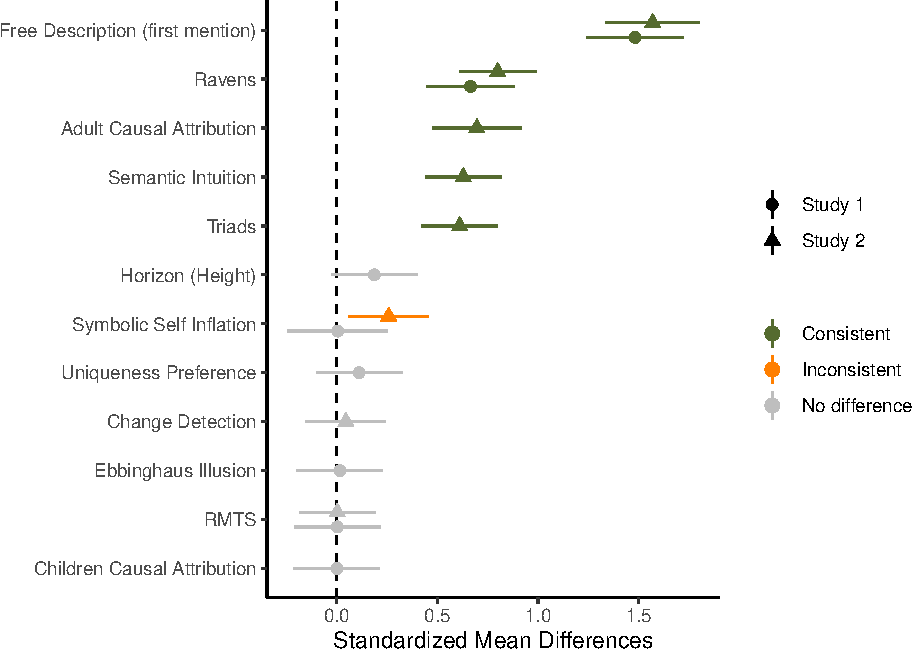
\includegraphics{CCRR_manuscript_files/figure-latex/unnamed-chunk-15-1.pdf}

As our first exploratory analysis, we identified the key effect of interest from our pre-registration (usually a main effect of culture or an interaction of culture, depending on task) and converted the coefficient into a standardized measure of effect size (standardized mean difference; SMD) via the method described by (2014). Because there is no ``correct'' direction for all of the tasks except Raven's Matrices, we show the absolute value of the effect size. Figure FIXME shows these effect sizes.

Across our two experiments, we saw consistent and generally large differences (SMD \textgreater{} 0.6) in Free Description, Raven's Matrices, Adult Causal Attribution, Semantic Intuition and Triads tasks. Aside from Raven's Matrices, all of these tasks had in common that they were deliberative linguistic tasks that tapped into relatively high-level cognitive constructs. In contrast, we observed effect sizes close to zero for our more aesthetic and perceptual tasks (Change Detection, Ebbinghaus Illusion, and Horizon). We also observed little consistent difference in four other tasks (RMTS, Symbolic Self-Inflation, Uniqueness Preference, and Children's Causal Attribution), perhaps for reasons idiosyncratic to each. We return to the broader question of generalization across task types in the General Discussion.

\hypertarget{reliability-assessment}{%
\subsection{Reliability assessment}\label{reliability-assessment}}

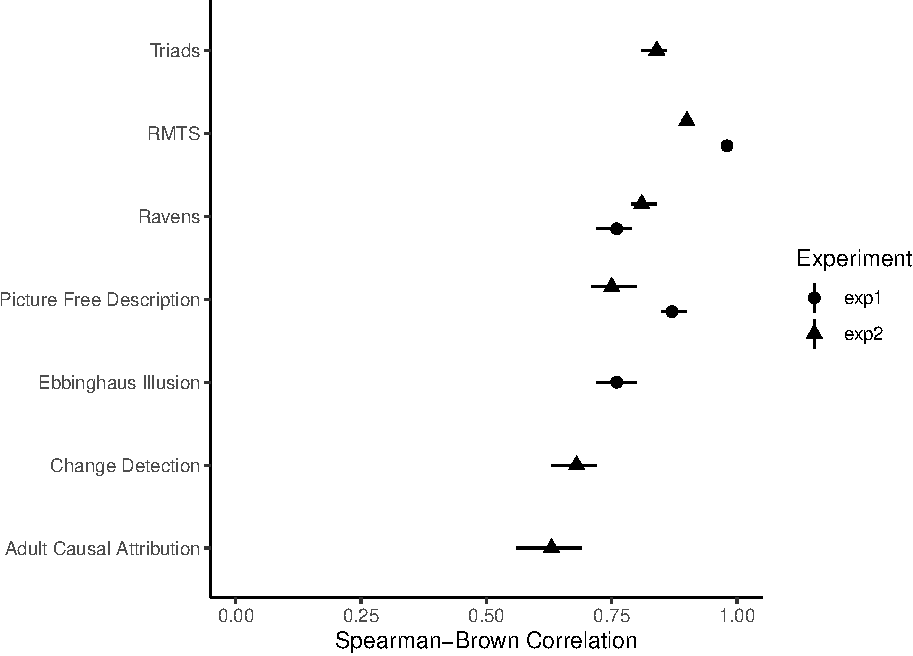
\includegraphics{CCRR_manuscript_files/figure-latex/unnamed-chunk-16-1.pdf}

One question motivating our work was whether the individual tasks we used were reliable enough -- had low enough measurement error -- to be used for further investigation of individual differences. The gold standard for the measurement of whether a task yields stable within-person measurements is test-retest reliability (simply because test-retest gives a direct estimate of stability over time), but this method was outside the scope of our study. Thus we used a split-half approach, asking whether participants' answers on individual questions related to one another. We used a permutation-based split half approach (Parsons, 2021) in which we made 5000 random splits of items into two simulated ``halves'' and then computed the within-person correlation between scores on these two halves, averaging across simulated runs. To estimate the reliability of the full-length instrument, we used the Spearman-Brown ``prophecy'' formula.

Since split-half approach is only suitable for tasks with multiple trials, we thus dropped the tasks with less than four trials from the analysis. For tasks with more than one condition, we focused on the conditions that were predicted to show cultural differences (i.e.~Illusion context condition for Ebbinghaus task; Situational judgements for Adult Causal Attribution task; Context condition for Change Detection task).

Figure FIXME shows the corrected split-half reliabilities for all tasks in both of our experiments. Overall the reliabilities are high (all Spearman-Brown Correlations \textgreater{} 0.6). We further investigated whether there was cultural variation in the reliability of tasks. For most tasks, the reliabilities were relatively similar (within 0.1 of one another), with no systematic pattern of greater reliabilities for either culture. The only exceptions were Change Detection (\emph{US - CN} = -0.19), Adult Causal Attribution (\emph{US - CN} = -0.19), Free Description in Study 1 (\emph{US - CN} = -0.23).

\hypertarget{relations-between-individual-tasks}{%
\subsection{Relations between individual tasks}\label{relations-between-individual-tasks}}

One (perhaps simplistic) interpretation of the prior literature on cultural variation is that there is a general tendency toward holistic or analytic reasoning that varies across cultures and explains variation in tasks. This single dimension might correspond to broad (or focused) attention and contextualized, relational reasoning (or an emphasis on focal people or objects). As a first step towards investigating this interpretation, we explored whether there was a single dimension of cross-cultural variation in our data. We treated the missing data using two approaches: listwise deletion and imputation with means. Two approaches yielded comparable results with the correlation values, so here we reported correlations from listwise deletion.

Correlations between task scores were quite low on average, however, suggesting limited support for this hypothesis. Across both Experiments 1 and 2, the largest correlations observed were -0.29 (Triads and Adult Causal Attribution in study 2) and -0.28 (Free Description and Ravens in Study 2), and -0.24 (Adult Causal Attribution and Free Description in Study 2) All other correlations were between -0.23 and 0.23. Hence, the amount of shared variation between tasks was quite limited and our attempts at exploratory factor analysis discovered structures with many distinct factors and very low loading on the first factor. We did not pursue this direction further though we welcome further explorations of this type using our dataset.

\hypertarget{demographic-variation-and-explicit-measures-of-cultural-identity}{%
\subsection{Demographic variation and explicit measures of cultural identity}\label{demographic-variation-and-explicit-measures-of-cultural-identity}}

Does demographic or variation in cultural identity predict responding in our tasks? Our approach to this question was to fit a set of exploratory regression models for each task, predicting task scores as a function of an individual scale and its interaction with culture. This approach allowed us to explore both within- and across-culture effects in a single model. Our predictors were 1) the summed score for our global/local cultural identity and consumption measures (with local items reverse-scored, such that higher scores represent more global identity and consumption patterns), 2) geographic information about where participants grew up (specifically, regions that have historically farmed primarily rice or wheat in China, following (2014), and culturally distinct regions of the US following FIXME), and 3) a range of demographic factors, {[}FIXME{]} including age, gender identity, subjective socioeconomic status measured using the MacArthur Ladder, level of maternal education, residential mobility{[}FIXME{]}, and number of international experiences.

\hypertarget{task-global-identity-relationships}{%
\subsubsection{Task-Global identity relationships}\label{task-global-identity-relationships}}

We fit the global-local identity models for tasks in Experiment 2 since we did not collect these scales in Experiment 1. We include the coefficients for all models in Supplementary Table FIXME Two of these relationships were statistically significant at .01 \textless{} p \textless{} .05 (Adult Causal Attribution task and Triads task) but neither of these relationships were particularly strong and they would not survive any appropriate correction for multiple comparisons.

\hypertarget{task-geographic-origin-relationships}{%
\subsubsection{Task-Geographic origin relationships}\label{task-geographic-origin-relationships}}

We considered whether regions within each country were meaningful predictors for task performance. For China, regions were categorized as rice-cultivating regions and wheat-cultivating regions based on FIXME. For U.S. regions were categorized as either FIXME. We fit the region models for tasks in Experiment 1 and Experiment 2 separately, and coefficients for all models were included in the Supplementary Table FIXME. One relationship in Experiment 1 (Coast for Free Description in U.S) and four relationships in Experiment 2 (Coast and Region for Ravens in U.S; Coast and Region for Change Detection in U.S) were statistically significant at .01 \textless{} p \textless{} .05. But none survived Bonferroni correction for multiple comparisons.

\hypertarget{basic-demographic-effects}{%
\subsubsection{Basic demographic effects}\label{basic-demographic-effects}}

\begin{verbatim}
## [1] "overseaexpnum" "objectiveses"  "subjectiveses" "age"          
## [5] "gender"        "stem_or_not"
\end{verbatim}

\begin{verbatim}
## # A tibble: 13 x 10
## # Groups:   culture, task_name, study, demog_type [13]
##    culture task_name study demog_type    term  estimate std.e~1 stati~2  p.value
##    <chr>   <chr>     <chr> <chr>         <chr>    <dbl>   <dbl>   <dbl>    <dbl>
##  1 CN      RMTS      d1    age           demo~  2.21e-2 8.91e-3    2.48 1.42e- 2
##  2 CN      SI        d1    age           demo~  2.64e-2 1.26e-2    2.09 3.83e- 2
##  3 US      RV        d2    age           demo~ -2.37e-3 1.19e-3   -1.99 4.75e- 2
##  4 CN      CD        d2    age           demo~  2.87e+2 9.51e+1    3.01 3.02e- 3
##  5 US      CD        d2    age           demo~  1.32e+2 1.75e+1    7.51 1.10e-12
##  6 CN      CA        d1    objectiveses  demo~ -7.69e-2 3.84e-2   -2.00 4.67e- 2
##  7 CN      CD        d2    overseaexpnum demo~ -1.18e+3 4.59e+2   -2.58 1.08e- 2
##  8 US      SeI       d2    overseaexpnum demo~  3.30e-2 1.54e-2    2.15 3.27e- 2
##  9 US      CP        d1    subjectiveses demo~ -5.50e-2 2.00e-2   -2.75 6.65e- 3
## 10 CN      RMTS      d2    subjectiveses demo~ -4.01e-2 1.95e-2   -2.05 4.16e- 2
## 11 US      RV        d2    subjectiveses demo~ -2.01e-2 9.38e-3   -2.14 3.32e- 2
## 12 CN      CD        d2    subjectiveses demo~ -7.36e+2 2.21e+2   -3.33 1.10e- 3
## 13 CN      TD        d2    subjectiveses demo~ -2.57e-2 1.26e-2   -2.05 4.23e- 2
## # ... with 1 more variable: p.adjusted <dbl>, and abbreviated variable names
## #   1: std.error, 2: statistic
\end{verbatim}

\begin{verbatim}
## # A tibble: 8 x 10
## # Groups:   culture, task_name, study, demog_type [8]
##   culture task_name study demog~1 term  estimate std.e~2 stati~3 p.value p.adj~4
##   <chr>   <chr>     <chr> <chr>   <chr>    <dbl>   <dbl>   <dbl>   <dbl>   <dbl>
## 1 CN      RV        d2    gender  demo~ -1.17e-1 3.42e-2   -3.43 7.43e-4   0.113
## 2 US      CD        d2    gender  demo~  5.15e+3 2.33e+3    2.21 2.81e-2   1    
## 3 CN      CA        d2    gender  demo~  5.01e-1 2.02e-1    2.48 1.47e-2   1    
## 4 CN      TD        d2    gender  demo~ -3.36e-1 1.59e-1   -2.11 3.63e-2   1    
## 5 CN      FD        d2    stem_o~ demo~  1.09e-1 5.01e-2    2.17 3.18e-2   1    
## 6 US      RV        d2    stem_o~ demo~  9.79e-2 3.49e-2    2.81 5.36e-3   0.815
## 7 CN      CA        d2    stem_o~ demo~  4.83e-1 2.11e-1    2.29 2.37e-2   1    
## 8 US      TD        d2    stem_o~ demo~  6.32e-2 2.88e-2    2.20 2.89e-2   1    
## # ... with abbreviated variable names 1: demog_type, 2: std.error,
## #   3: statistic, 4: p.adjusted
\end{verbatim}

\begin{verbatim}
## # A tibble: 1 x 10
## # Groups:   culture, task_name, study, demog_type [1]
##   culture task_n~1 study demog~2 term  estim~3 std.e~4 stati~5  p.value p.adju~6
##   <chr>   <chr>    <chr> <chr>   <chr>   <dbl>   <dbl>   <dbl>    <dbl>    <dbl>
## 1 US      CD       d2    age     demo~    132.    17.5    7.51 1.10e-12 2.47e-10
## # ... with abbreviated variable names 1: task_name, 2: demog_type, 3: estimate,
## #   4: std.error, 5: statistic, 6: p.adjusted
\end{verbatim}

\begin{verbatim}
## # A tibble: 0 x 10
## # Groups:   culture, task_name, study, demog_type [0]
## # ... with 10 variables: culture <chr>, task_name <chr>, study <chr>,
## #   demog_type <chr>, term <chr>, estimate <dbl>, std.error <dbl>,
## #   statistic <dbl>, p.value <dbl>, p.adjusted <dbl>
\end{verbatim}

\setlength{\parindent}{-0.5in}
\setlength{\leftskip}{0.5in}

\newpage

\hypertarget{references}{%
\section{References}\label{references}}

\hypertarget{refs}{}
\begin{CSLReferences}{1}{0}
\leavevmode\vadjust pre{\hypertarget{ref-adler2000relationship}{}}%
Adler, N. E., Epel, E. S., Castellazzo, G., \& Ickovics, J. R. (2000). Relationship of subjective and objective social status with psychological and physiological functioning. \emph{Health Psychology}, \emph{19}(6), 586.

\leavevmode\vadjust pre{\hypertarget{ref-arnett2016neglected}{}}%
Arnett, J. J. (2016). The neglected 95\%: Why american psychology needs to become less american.

\leavevmode\vadjust pre{\hypertarget{ref-bailey1997conceptions}{}}%
Bailey, J. R., Chen, C. C., \& Dou, S.-G. (1997). Conceptions of self and performance-related feedback in the US, japan and china. \emph{J Int Bus Stud}, \emph{28}(3), 605--625.

\leavevmode\vadjust pre{\hypertarget{ref-barr2013random}{}}%
Barr, D. J., Levy, R., Scheepers, C., \& Tily, H. J. (2013). Random effects structure for confirmatory hypothesis testing: Keep it maximal. \emph{Journal of Memory and Language}, \emph{68}(3), 255--278.

\leavevmode\vadjust pre{\hypertarget{ref-blouin2004difference}{}}%
Blouin, D. C., \& Riopelle, A. J. (2004). The difference between t and z and the difference it makes. \emph{J of Gen Psych}, \emph{131}(1), 77--84.

\leavevmode\vadjust pre{\hypertarget{ref-burkner2017brms}{}}%
Bürkner, P.-C. (2017). Brms: An r package for bayesian multilevel models using stan. \emph{Journal of Statistical Software}, \emph{80}, 1--28.

\leavevmode\vadjust pre{\hypertarget{ref-carstensen2019context}{}}%
Carstensen, A., Zhang, J., Heyman, G. D., Fu, G., Lee, K., \& Walker, C. M. (2019). Context shapes early diversity in abstract thought. \emph{PNAS}, \emph{116}(28), 13891--13896.

\leavevmode\vadjust pre{\hypertarget{ref-chan2011english}{}}%
Chan, C. C., Tardif, T., Chen, J., Pulverman, R. B., Zhu, L., \& Meng, X. (2011). English-and chinese-learning infants map novel labels to objects and actions differently. \emph{Dev Psy}, \emph{47}(5), 1459.

\leavevmode\vadjust pre{\hypertarget{ref-cheng2020development}{}}%
Cheng, L. (2020). \emph{The development of cognitive styles among american and chinese children} (PhD thesis).

\leavevmode\vadjust pre{\hypertarget{ref-choi1999causal}{}}%
Choi, I., Nisbett, R. E., \& Norenzayan, A. (1999). Causal attribution across cultures. \emph{Psy Bull}, \emph{125}(1), 47.

\leavevmode\vadjust pre{\hypertarget{ref-chua2005cultural}{}}%
Chua, H. F., Boland, J. E., \& Nisbett, R. E. (2005). Cultural variation in eye movements during scene perception. \emph{PNAS}, \emph{102}(35), 12629--12633.

\leavevmode\vadjust pre{\hypertarget{ref-church2012self}{}}%
Church, A. T., Alvarez, J. M., Katigbak, M. S., Mastor, K. A., Cabrera, H. F., Tanaka-Matsumi, J., et al.others. (2012). Self-concept consistency and short-term stability in eight cultures. \emph{J Res Pers}, \emph{46}(5), 556--570.

\leavevmode\vadjust pre{\hypertarget{ref-church2014relating}{}}%
Church, A. T., Katigbak, M. S., Ibáñez-Reyes, J., Jesús Vargas-Flores, J. de, Curtis, G. J., Tanaka-Matsumi, J., et al.others. (2014). Relating self-concept consistency to hedonic and eudaimonic well-being in eight cultures. \emph{J Cross Cult Psy}, \emph{45}(5), 695--712.

\leavevmode\vadjust pre{\hypertarget{ref-cleveland2007acculturaton}{}}%
Cleveland, M., \& Laroche, M. (2007). Acculturaton to the global consumer culture: Scale development and research paradigm. \emph{Journal of Business Research}, \emph{60}(3), 249--259.

\leavevmode\vadjust pre{\hypertarget{ref-cleveland2015intersection}{}}%
Cleveland, M., Laroche, M., \& Takahashi, I. (2015). The intersection of global consumer culture and national identity and the effect on japanese consumer behavior. \emph{Journal of International Consumer Marketing}, \emph{27}(5), 364--387.

\leavevmode\vadjust pre{\hypertarget{ref-corriveau2017cultural}{}}%
Corriveau, K. H., DiYanni, C. J., Clegg, J. M., Min, G., Chin, J., \& Nasrini, J. (2017). Cultural differences in the imitation and transmission of inefficient actions. \emph{J Exp Child Psy}, \emph{161}, 1--18.

\leavevmode\vadjust pre{\hypertarget{ref-de2015jspsych}{}}%
De Leeuw, J. R. (2015). jsPsych: A JavaScript library for creating behavioral experiments in a web browser. \emph{Behavior Research Methods}, \emph{47}(1), 1--12.

\leavevmode\vadjust pre{\hypertarget{ref-diyanni2015role}{}}%
DiYanni, C. J., Corriveau, K. H., Kurkul, K., Nasrini, J., \& Nini, D. (2015). The role of consensus and culture in children's imitation of inefficient actions. \emph{J Exp Child Psy}, \emph{137}, 99--110.

\leavevmode\vadjust pre{\hypertarget{ref-doherty2008context}{}}%
Doherty, M. J., Tsuji, H., \& Phillips, W. A. (2008). The context sensitivity of visual size perception varies across cultures. \emph{Perception}, \emph{37}(9), 1426--1433.

\leavevmode\vadjust pre{\hypertarget{ref-duffy2009development}{}}%
Duffy, S., Toriyama, R., Itakura, S., \& Kitayama, S. (2009). Development of cultural strategies of attention in {N}orth {A}merican and {J}apanese children. \emph{J Exp Child Psy}, \emph{102}(3), 351--359.

\leavevmode\vadjust pre{\hypertarget{ref-flake2020measurement}{}}%
Flake, J. K., \& Fried, E. I. (2020). Measurement schmeasurement: Questionable measurement practices and how to avoid them. \emph{Advances in Methods and Practices in Psychological Science}, \emph{3}(4), 456--465.

\leavevmode\vadjust pre{\hypertarget{ref-goddu2018toddlers}{}}%
Goddu, M., \& Walker, C. M. (2018). Toddlers and adults simultaneously track multiple hypotheses in a causal learning task. In \emph{CogSci}.

\leavevmode\vadjust pre{\hypertarget{ref-henrich2010weirdest}{}}%
Henrich, J., Heine, S. J., \& Norenzayan, A. (2010). The weirdest people in the world? \emph{Behav Brain Sci}, \emph{33}(2-3), 61--83.

\leavevmode\vadjust pre{\hypertarget{ref-imada2013east}{}}%
Imada, T., Carlson, S. M., \& Itakura, S. (2013). East--west cultural differences in context-sensitivity are evident in early childhood. \emph{Dev Sci}, \emph{16}(2), 198--208.

\leavevmode\vadjust pre{\hypertarget{ref-ji2001culture}{}}%
Ji, L.-J., Nisbett, R. E., \& Su, Y. (2001). Culture, change, and prediction. \emph{Psych Sci}, \emph{12}(6), 450--456.

\leavevmode\vadjust pre{\hypertarget{ref-ji2000culture}{}}%
Ji, L.-J., Peng, K., \& Nisbett, R. E. (2000). Culture, control, and perception of relationships in the environment. \emph{JPSP}, \emph{78}(5), 943.

\leavevmode\vadjust pre{\hypertarget{ref-ji2004culture}{}}%
Ji, L.-J., Zhang, Z., \& Nisbett, R. E. (2004). Is it culture or is it language? \emph{JPSP}, \emph{87}(1), 57.

\leavevmode\vadjust pre{\hypertarget{ref-kim1999deviance}{}}%
Kim, H., \& Markus, H. R. (1999). Deviance or uniqueness, harmony or conformity? A cultural analysis. \emph{JPSP}, \emph{77}(4), 785.

\leavevmode\vadjust pre{\hypertarget{ref-kitayama2009cultural}{}}%
Kitayama, S., Park, H., Sevincer, A. T., Karasawa, M., \& Uskul, A. K. (2009). A cultural task analysis of implicit independence. \emph{JPSP}, \emph{97}(2), 236.

\leavevmode\vadjust pre{\hypertarget{ref-kuwabara2012cross}{}}%
Kuwabara, M., \& Smith, L. B. (2012). Cross-cultural differences in cognitive development: Attention to relations and objects. \emph{J Exp Child Psy}, \emph{113}(1), 20--35.

\leavevmode\vadjust pre{\hypertarget{ref-kwan1997pancultural}{}}%
Kwan, V. S., Bond, M. H., \& Singelis, T. M. (1997). Pancultural explanations for life satisfaction: Adding relationship harmony to self-esteem. \emph{JPSP}, \emph{73}(5), 1038.

\leavevmode\vadjust pre{\hypertarget{ref-li2018name}{}}%
Li, J., Liu, L., Chalmers, E., \& Snedeker, J. (2018). What is in a name?: The development of cross-cultural differences in referential intuitions. \emph{Cognition}, \emph{171}, 108--111.

\leavevmode\vadjust pre{\hypertarget{ref-liang2012effect}{}}%
Liang, B., \& He, Y. (2012). The effect of culture on consumer choice: The need for conformity vs. The need for uniqueness. \emph{Int J of Consum Stu}, \emph{36}(3), 352--359.

\leavevmode\vadjust pre{\hypertarget{ref-machery2020replication}{}}%
Machery, E. (2020). What is a replication? \emph{Philosophy of Science}, \emph{87}(4), 545--567.

\leavevmode\vadjust pre{\hypertarget{ref-markus1992and}{}}%
Markus, H. R., \& Kitayama, S. (1992). The what, why and how of cultural psychology: A review of shweder's thinking through cultures. \emph{Psychological Inquiry}, \emph{3}(4), 357--364.

\leavevmode\vadjust pre{\hypertarget{ref-markus2010cultures}{}}%
Markus, H. R., \& Kitayama, S. (2010). Cultures and selves: A cycle of mutual constitution. \emph{Perspectives on Psychological Science}, \emph{5}(4), 420--430.

\leavevmode\vadjust pre{\hypertarget{ref-masuda2006culture}{}}%
Masuda, T., \& Nisbett, R. E. (2006). Culture and change blindness. \emph{Cognitive Science}, \emph{30}(2), 381--399.

\leavevmode\vadjust pre{\hypertarget{ref-mercier2012use}{}}%
Mercier, H., Yama, H., Kawasaki, Y., Adachi, K., \& Van der Henst, J.-B. (2012). Is the use of averaging in advice taking modulated by culture? \emph{J Cog \& Culture}, \emph{12}(1-2), 1--16.

\leavevmode\vadjust pre{\hypertarget{ref-mercier2015easterners}{}}%
Mercier, H., Zhang, J., Qu, Y., Lu, P., \& Van der Henst, J.-B. (2015). Do easterners and westerners treat contradiction differently? \emph{J Cog \& Culture}, \emph{15}(1-2), 45--63.

\leavevmode\vadjust pre{\hypertarget{ref-moriguchi2012cultural}{}}%
Moriguchi, Y., Evans, A. D., Hiraki, K., Itakura, S., \& Lee, K. (2012). Cultural differences in the development of cognitive shifting. \emph{J Exp Child Psy}, \emph{111}(2), 156--163.

\leavevmode\vadjust pre{\hypertarget{ref-morris1995causal}{}}%
Morris, M. W., Nisbett, R. E., \& Peng, K. (1995). Causal attribution across domains and cultures.

\leavevmode\vadjust pre{\hypertarget{ref-morris1994culture}{}}%
Morris, M. W., \& Peng, K. (1994). Culture and cause: American and chinese attributions for social and physical events. \emph{JPSP}, \emph{67}(6), 949.

\leavevmode\vadjust pre{\hypertarget{ref-muthukrishna2020beyond}{}}%
Muthukrishna, M., Bell, A. V., Henrich, J., Curtin, C. M., Gedranovich, A., McInerney, J., \& Thue, B. (2020). Beyond WEIRD psychology: Measuring and mapping scales of cultural and psychological distance. \emph{Psych Sci}, \emph{31}(6), 678--701.

\leavevmode\vadjust pre{\hypertarget{ref-na2010cultural}{}}%
Na, J., Grossmann, I., Varnum, M. E., Kitayama, S., Gonzalez, R., \& Nisbett, R. E. (2010). Cultural differences are not always reducible to individual differences. \emph{PNAS}, \emph{107}(14), 6192--6197.

\leavevmode\vadjust pre{\hypertarget{ref-nielsen2017persistent}{}}%
Nielsen, M., Haun, D., Kärtner, J., \& Legare, C. H. (2017). The persistent sampling bias in developmental psychology: A call to action. \emph{J Exp Child Psy}, \emph{162}, 31--38.

\leavevmode\vadjust pre{\hypertarget{ref-nosek2020replication}{}}%
Nosek, B. A., \& Errington, T. M. (2020). What is replication? \emph{PLoS Biology}, \emph{18}(3), e3000691.

\leavevmode\vadjust pre{\hypertarget{ref-open2015estimating}{}}%
Open Science Collaboration. (2015). Estimating the reproducibility of psychological science. \emph{Science}, \emph{349}(6251).

\leavevmode\vadjust pre{\hypertarget{ref-parsons2021splithalf}{}}%
Parsons, S. (2021). Splithalf: Robust estimates of split half reliability. \emph{Journal of Open Source Software}, \emph{6}(60), 3041.

\leavevmode\vadjust pre{\hypertarget{ref-richland2010young}{}}%
Richland, L. E., Chan, T.-K., Morrison, R. G., \& Au, T. K.-F. (2010). Young children's analogical reasoning across cultures: Similarities and differences. \emph{J Exp Child Psy}, \emph{105}(1-2), 146--153.

\leavevmode\vadjust pre{\hypertarget{ref-sabbagh2006development}{}}%
Sabbagh, M. A., Xu, F., Carlson, S. M., Moses, L. J., \& Lee, K. (2006). The development of executive functioning and theory of mind: A comparison of chinese and US preschoolers. \emph{Psych Sci}, \emph{17}(1), 74--81.

\leavevmode\vadjust pre{\hypertarget{ref-seiver2013did}{}}%
Seiver, E., Gopnik, A., \& Goodman, N. D. (2013). Did she jump because she was the big sister or because the trampoline was safe? \emph{Child Dev}, \emph{84}(2), 443--454.

\leavevmode\vadjust pre{\hypertarget{ref-senzaki2014holistic}{}}%
Senzaki, S., Masuda, T., \& Nand, K. (2014). Holistic versus analytic expressions in artworks: Cross-cultural differences and similarities in drawings and collages by {C}anadian and {J}apanese school-age children. \emph{J Cross Cult Psy}, \emph{45}(8), 1297--1316.

\leavevmode\vadjust pre{\hypertarget{ref-simmons2011}{}}%
Simmons, J. P., Nelson, L. D., \& Simonsohn, U. (2011). False-positive psychology. \emph{Psych Sci}, \emph{22}(11), 1359--1366.

\leavevmode\vadjust pre{\hypertarget{ref-spencer2009dialectical}{}}%
Spencer-Rodgers, J., Boucher, H. C., Mori, S. C., Wang, L., \& Peng, K. (2009). The dialectical self-concept. \emph{Pers Soc Psy B}, \emph{35}(1), 29--44.

\leavevmode\vadjust pre{\hypertarget{ref-spencer2009cultural}{}}%
Spencer-Rodgers, J., Boucher, H. C., Peng, K., \& Wang, L. (2009). Cultural differences in self-verification. \emph{J Exp Soc Psy}, \emph{45}(4), 860--866.

\leavevmode\vadjust pre{\hypertarget{ref-spencer2007culture}{}}%
Spencer-Rodgers, J., Williams, M. J., Hamilton, D. L., Peng, K., \& Wang, L. (2007). Culture and group perception: Dispositional and stereotypic inferences about novel and national groups. \emph{JPSP}, \emph{93}(4), 525.

\leavevmode\vadjust pre{\hypertarget{ref-su2020analogical}{}}%
Su, S. (2020). \emph{Analogical reasoning in {C}hinese and {US} adults} (Master's thesis). Cornell University.

\leavevmode\vadjust pre{\hypertarget{ref-talhelm2014large}{}}%
Talhelm, T., Zhang, X., Oishi, S., Shimin, C., Duan, D., Lan, X., \& Kitayama, S. (2014). Large-scale psychological differences within {C}hina explained by rice versus wheat agriculture. \emph{Science}, \emph{344}(6184), 603--608.

\leavevmode\vadjust pre{\hypertarget{ref-tan2020chinese}{}}%
Tan, B. (2020). \emph{Chinese and US young children's executive function and its sociocultural antecedents} (PhD thesis). The University of Memphis.

\leavevmode\vadjust pre{\hypertarget{ref-tardif1996nouns}{}}%
Tardif, T. (1996). Nouns are not always learned before verbs: Evidence from mandarin speakers' early vocabularies. \emph{Dev Psy}, \emph{32}(3), 492.

\leavevmode\vadjust pre{\hypertarget{ref-waxman2016early}{}}%
Waxman, S. R., Fu, X., Ferguson, B., Geraghty, K., Leddon, E., Liang, J., \& Zhao, M.-F. (2016). How early is infants' attention to objects and actions shaped by culture? New evidence from 24-month-olds raised in the US and china. \emph{Front Psy}, \emph{7}, 97.

\leavevmode\vadjust pre{\hypertarget{ref-westfall2014statistical}{}}%
Westfall, J., Kenny, D. A., \& Judd, C. M. (2014). Statistical power and optimal design in experiments in which samples of participants respond to samples of stimuli. \emph{Journal of Experimental Psychology: General}, \emph{143}(5), 2020.

\leavevmode\vadjust pre{\hypertarget{ref-yamagishi2008preferences}{}}%
Yamagishi, T., Hashimoto, H., \& Schug, J. (2008). Preferences versus strategies as explanations for culture-specific behavior. \emph{Psychological Science}, \emph{19}(6), 579--584.

\leavevmode\vadjust pre{\hypertarget{ref-zhou2008perceiving}{}}%
Zhou, J., Gotch, C., Zhou, Y., \& Liu, Z. (2008). Perceiving an object in its context---is the context cultural or perceptual? \emph{Journal of Vision}, \emph{8}(12), 2--2.

\leavevmode\vadjust pre{\hypertarget{ref-zwaan2018making}{}}%
Zwaan, R. A., Etz, A., Lucas, R. E., \& Donnellan, M. B. (2018). Making replication mainstream. \emph{Behavioral and Brain Sciences}, \emph{41}.

\end{CSLReferences}


\end{document}
